% answers.tex —— 1977 年·四川卷 · 参考答案与详细解析片段
% 由 tools/generate_projects.py 依来源总账自 1977/1977_数学真题_四川_试题.md + 1977/1977_数学真题_四川_解析正文.md + 1977/1977_数学真题_四川_答案要点.md 生成，勿手改（改源 MD 后重跑）


\begin{gktip}
固定源《四川1977年高考数学试题解》是题面与解答连续出现的扫描材料（PDF 第 1—8 页，书籍页码 128—135）。下文逐题对照源解答并重新计算关键结论；第 6 题与参考题的小题原卷印作“1．”“2．”“3．”，已按本库小问连续编号规范重排为（1）（2）（3）；参考题 1（2）的源解答中间步有一处排印失误（和差化积后印作 $1+\cos2t$，按其后一行积分结果应为 $1-\cos2t$），不影响最终结论，相应位置已留注。
\end{gktip}

\begin{answer}
\gksolhead{1}{}

\textbf{题目}：

（1） 解方程：$9(3x+2)^2-4=0$。（8 分）

（2） 已知 $\operatorname{Lg}5=0.6990$，问 $8^{34}\times25^{11}$ 是多少位的整数？（8 分）

（3） 把 $\sin(30^\circ+x)+\cos(x+60^\circ)-\sin^2x-\cos^2x$ 化成积的形式。（8 分）

\Needspace{5\baselineskip}
（4） 试证明：

\nopagebreak[4]
\[
\bigl[(2m)^0-(m+x)^{-2}\bigr]\div\bigl[(2x)^0-(m+x)^{-1}\bigr]^2\cdot\Bigl[2m^0-\frac{1-(m-x)^2}{2mx}\Bigr]=\frac{(m+x+1)^2}{2mx}.
\]

（8 分）

\Needspace{4\baselineskip}
\textbf{解析}

\gksubpart{（1）}

\Needspace{5\baselineskip}
移项得 $9(3x+2)^2=4$。由平方差公式把左端因式分解：

\nopagebreak[4]
\[
\bigl[3(3x+2)\bigr]^2-2^2=\bigl[3(3x+2)+2\bigr]\bigl[3(3x+2)-2\bigr]=(9x+8)(9x+4)=0,
\]

\Needspace{5\baselineskip}
所以 $9x+8=0$ 或 $9x+4=0$，即

\nopagebreak[4]
\[
x_1=-\frac89,\qquad x_2=-\frac49.
\]

\gksubpart{（2）}

\Needspace{5\baselineskip}
设 $N=8^{34}\times25^{11}$。利用 $8=2^3$、$25=5^2$ 与 $\operatorname{Lg}2+\operatorname{Lg}5=\operatorname{Lg}10=1$：

\nopagebreak[4]
\[
\operatorname{Lg}N=34\operatorname{Lg}8+11\operatorname{Lg}25
=102\operatorname{Lg}2+22\operatorname{Lg}5
=102(1-\operatorname{Lg}5)+22\operatorname{Lg}5
=102-80\operatorname{Lg}5.
\]

\Needspace{5\baselineskip}
代入 $\operatorname{Lg}5=0.6990$：

\nopagebreak[4]
\[
\operatorname{Lg}N=102-80\times0.6990=102-55.92=46.08.
\]

对数首数为 $46$，故 $N$ 是 $47$ 位的整数。

\gksubpart{（3）}

\Needspace{5\baselineskip}
先化余弦为正弦：$\cos(x+60^\circ)=\sin\bigl[90^\circ-(x+60^\circ)\bigr]=\sin(30^\circ-x)$。于是

\nopagebreak[4]
\[
\begin{aligned}
&\sin(30^\circ+x)+\cos(x+60^\circ)-\sin^2x-\cos^2x\\
&=\sin(30^\circ+x)+\sin(30^\circ-x)-1\\
&=2\sin\frac{(30^\circ+x)+(30^\circ-x)}2\cos\frac{(30^\circ+x)-(30^\circ-x)}2-1\\
&=2\sin30^\circ\cos x-1=\cos x-1=-(1-\cos x)
=-2\sin^2\frac x2.
\end{aligned}
\]

\gksubpart{（4）}

\Needspace{5\baselineskip}
原卷第三个中括号印作 $2m^0$（与第一个中括号的 $(2m)^0$ 不同），按 $2m^0=2$ 化简。记 $u=m+x$，则

\nopagebreak[4]
\[
(2m)^0-(m+x)^{-2}=1-\frac1{u^2}=\frac{(u-1)(u+1)}{u^2},
\]

\nopagebreak[4]
\[
\bigl[(2x)^0-(m+x)^{-1}\bigr]^2=\Bigl(1-\frac1u\Bigr)^2=\frac{(u-1)^2}{u^2},
\]

\nopagebreak[4]
\[
2m^0-\frac{1-(m-x)^2}{2mx}
=2-\frac{1-(m-x)^2}{2mx}
=\frac{4mx-1+(m-x)^2}{2mx}
=\frac{u^2-1}{2mx}
=\frac{(u-1)(u+1)}{2mx}.
\]

\Needspace{5\baselineskip}
三者相乘（前两个因子作除法）：

\nopagebreak[4]
\[
\frac{(u-1)(u+1)}{u^2}\div\frac{(u-1)^2}{u^2}\cdot\frac{(u-1)(u+1)}{2mx}
=\frac{(u+1)^2}{2mx}
=\frac{(m+x+1)^2}{2mx}.
\]

等于右端，恒等式获证。

\gkanswer{答案（1）：$x=-\dfrac49$ 或 $x=-\dfrac89$。}

\gkanswer{答案（2）：$8^{34}\times25^{11}$ 是 $47$ 位的整数。}

\gkanswer{答案（3）：$-2\sin^2\dfrac x2$。}

\gkanswer{答案（4）：见解析版}

\end{answer}
\begin{answer}
\gksolhead{2}{}

\textbf{题目}（10 分）：

将半径为 $R$，中心角为 $120^\circ$ 的扇形铁片，卷成一圆锥容器，问圆锥容器的容积是多少？（接缝及卷边不计）

\begin{gktip}
原源 PDF 第 3 页附有扇形卷成圆锥的示意图（标 $R$、$r$、$h$、弧长记号 $C$ 与 $120^\circ$ 圆心角）；LaTeX 版按源图重绘。
\end{gktip}
\nopagebreak[4]
\begin{center}% 1977 年四川卷第二题：半径 R、中心角 120° 的扇形卷成圆锥容器
% 扇形顶点在左、弧张向右下（标弧长 C、圆心角 120°），
% 圆锥立在其上（虚线标高 h 与底面半径 r，母线即扇形半径 R）（按源卷第 3 页布局）
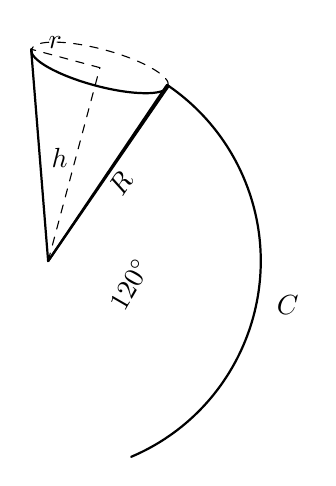
\begin{tikzpicture}[scale=0.9,line cap=round]
  % 圆锥（锥顶与扇形顶点重合）
  \coordinate (V) at (0,0);
  \coordinate (M) at (0.73,2.73);   % 底面椭圆中心（h=2.83，沿 75° 轴）
  \coordinate (P1) at (-0.24,2.99); % 底面椭圆左端
  \coordinate (P2) at (1.70,2.47);  % 底面椭圆右端（与扇形上半径共线）
  \draw[thick] (V)--(P1);
  \draw[thick] (V)--(P2);
  \begin{scope}[shift={(0.73,2.73)},rotate=-15]
    \draw[dashed] (1,0) arc (0:180:1 and 0.26);   % 底面椭圆后半（虚线）
    \draw[thick] (-1,0) arc (180:360:1 and 0.26); % 底面椭圆前半（实线）
\end{scope}
  % 高 h 与底面半径 r（虚线）
  \draw[dashed] (V)--(M);
  \node at (0.16,1.45) {$h$};
  \draw[dashed] (M)--(P1);
  \node at (0.10,3.08) {$r$};
  % 扇形（上半径与圆锥母线 V-P2 重合，标 R；下半径向右下，标弧长记号 C）
  \draw[thick] (V)--(56:3);
  \draw[thick] (-67:3) arc[start angle=-67, end angle=56, radius=3];
  \node[rotate=56] at (1.02,1.10) {$R$};
  \node[rotate=60] at (1.15,-0.32) {$120^\circ$};
  \node at (3.38,-0.62) {$C$};
\end{tikzpicture}
\end{center}
\nopagebreak[4]
\Needspace{4\baselineskip}
\textbf{解析}
\nopagebreak[4]
\begin{center}% 1977 年四川卷第二题：半径 R、中心角 120° 的扇形卷成圆锥容器
% 扇形顶点在左、弧张向右下（标弧长 C、圆心角 120°），
% 圆锥立在其上（虚线标高 h 与底面半径 r，母线即扇形半径 R）（按源卷第 3 页布局）
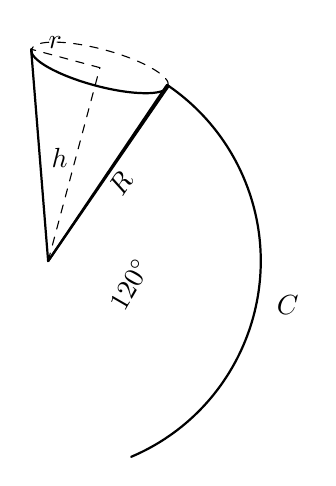
\begin{tikzpicture}[scale=0.9,line cap=round]
  % 圆锥（锥顶与扇形顶点重合）
  \coordinate (V) at (0,0);
  \coordinate (M) at (0.73,2.73);   % 底面椭圆中心（h=2.83，沿 75° 轴）
  \coordinate (P1) at (-0.24,2.99); % 底面椭圆左端
  \coordinate (P2) at (1.70,2.47);  % 底面椭圆右端（与扇形上半径共线）
  \draw[thick] (V)--(P1);
  \draw[thick] (V)--(P2);
  \begin{scope}[shift={(0.73,2.73)},rotate=-15]
    \draw[dashed] (1,0) arc (0:180:1 and 0.26);   % 底面椭圆后半（虚线）
    \draw[thick] (-1,0) arc (180:360:1 and 0.26); % 底面椭圆前半（实线）
\end{scope}
  % 高 h 与底面半径 r（虚线）
  \draw[dashed] (V)--(M);
  \node at (0.16,1.45) {$h$};
  \draw[dashed] (M)--(P1);
  \node at (0.10,3.08) {$r$};
  % 扇形（上半径与圆锥母线 V-P2 重合，标 R；下半径向右下，标弧长记号 C）
  \draw[thick] (V)--(56:3);
  \draw[thick] (-67:3) arc[start angle=-67, end angle=56, radius=3];
  \node[rotate=56] at (1.02,1.10) {$R$};
  \node[rotate=60] at (1.15,-0.32) {$120^\circ$};
  \node at (3.38,-0.62) {$C$};
\end{tikzpicture}
\end{center}
\nopagebreak[4]
\Needspace{5\baselineskip}
设卷成的圆锥底面半径为 $r$，高为 $h$。扇形的弧长

\nopagebreak[4]
\[
C=\frac{120\pi R}{180}=\frac{2\pi}3R.
\]

\Needspace{5\baselineskip}
卷成圆锥后，扇形弧长恰为底面圆周长：

\nopagebreak[4]
\[
2\pi r=\frac{2\pi}3R
\qquad\Longrightarrow\qquad
r=\frac13R.
\]

\Needspace{5\baselineskip}
圆锥的母线长等于扇形半径 $R$，由勾股定理，

\nopagebreak[4]
\[
h=\sqrt{R^2-r^2}=\sqrt{R^2-\Bigl(\frac R3\Bigr)^2}
=\frac{2\sqrt2}3R.
\]

\Needspace{5\baselineskip}
所以圆锥容积

\nopagebreak[4]
\[
V=\frac13\pi r^2h
=\frac13\pi\Bigl(\frac R3\Bigr)^2\cdot\frac{2\sqrt2}3R
=\frac{2\sqrt2}{81}\pi R^3.
\]

\gkanswer{答案：圆锥容器的容积为 $\dfrac{2\sqrt2}{81}\pi R^3$。}

\end{answer}
\begin{answer}
\gksolhead{3}{}

\textbf{题目}：

如图，$AD\text{、}BD$ 分别为 $\triangle ABC$ 的角平分线，延长 $AD$ 交 $\triangle ABC$ 的外接园于 $E$，连接 $BE$，求证：$BE=DE$。

\begin{gktip}
原源 PDF 第 3 页附有 $\triangle ABC$ 外接园示意图，弧上标有记号 1、2、3、4；LaTeX 版按源图重绘。
\end{gktip}
\nopagebreak[4]
\begin{center}% 1977 年四川卷第三题：△ABC 的外接园，AD、BD 为角平分线，
% AD 延长交园于 E，BD 延长交园于 F，求证 BE=DE；
% 弧上记号：1（弧BE）、2（弧EC）、3（弧CF）、4（弧AF）（按源卷第 3 页布局）
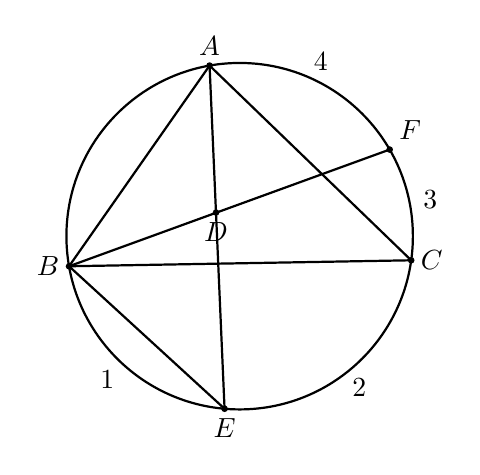
\begin{tikzpicture}[scale=1.0]
  \coordinate (A) at (100:2.2);
  \coordinate (F) at (30:2.2);
  \coordinate (C) at (-8:2.2);
  \coordinate (E) at (265:2.2);
  \coordinate (B) at (190:2.2);
  \coordinate (D) at (-0.30,0.30); % AE 与 BF 的交点
  \draw[thick] (0,0) circle (2.2);
  \draw[thick] (A)--(B)--(C)--cycle;
  \draw[thick] (A)--(E);
  \draw[thick] (B)--(F);
  \draw[thick] (B)--(E);
  \fill (A) circle (1.2pt) node[above] {$A$};
  \fill (B) circle (1.2pt) node[left] {$B$};
  \fill (C) circle (1.2pt) node[right] {$C$};
  \fill (D) circle (1.2pt) node[below] {$D$};
  \fill (E) circle (1.2pt) node[below] {$E$};
  \fill (F) circle (1.2pt) node[above right] {$F$};
  \node at (-1.68,-1.82) {$1$};
  \node at (1.52,-1.92) {$2$};
  \node at (2.42,0.46) {$3$};
  \node at (1.03,2.22) {$4$};
\end{tikzpicture}
\end{center}
\nopagebreak[4]
\Needspace{4\baselineskip}
\textbf{解析}
\nopagebreak[4]
\begin{center}% 1977 年四川卷第三题：△ABC 的外接园，AD、BD 为角平分线，
% AD 延长交园于 E，BD 延长交园于 F，求证 BE=DE；
% 弧上记号：1（弧BE）、2（弧EC）、3（弧CF）、4（弧AF）（按源卷第 3 页布局）
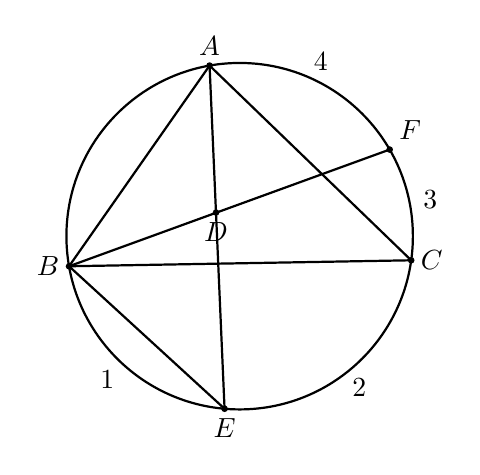
\begin{tikzpicture}[scale=1.0]
  \coordinate (A) at (100:2.2);
  \coordinate (F) at (30:2.2);
  \coordinate (C) at (-8:2.2);
  \coordinate (E) at (265:2.2);
  \coordinate (B) at (190:2.2);
  \coordinate (D) at (-0.30,0.30); % AE 与 BF 的交点
  \draw[thick] (0,0) circle (2.2);
  \draw[thick] (A)--(B)--(C)--cycle;
  \draw[thick] (A)--(E);
  \draw[thick] (B)--(F);
  \draw[thick] (B)--(E);
  \fill (A) circle (1.2pt) node[above] {$A$};
  \fill (B) circle (1.2pt) node[left] {$B$};
  \fill (C) circle (1.2pt) node[right] {$C$};
  \fill (D) circle (1.2pt) node[below] {$D$};
  \fill (E) circle (1.2pt) node[below] {$E$};
  \fill (F) circle (1.2pt) node[above right] {$F$};
  \node at (-1.68,-1.82) {$1$};
  \node at (1.52,-1.92) {$2$};
  \node at (2.42,0.46) {$3$};
  \node at (1.03,2.22) {$4$};
\end{tikzpicture}
\end{center}
\nopagebreak[4]
延长 $BD$ 交外接园于 $F$。由圆周角定理的推论（等弧对等角）：

\begin{itemize}
\item $AD$ 平分 $\angle BAC$，$E$ 在园上，故 $\overset{\frown}{BE}=\overset{\frown}{EC}$（图中弧记号 $1$ 与 $2$）；
\item $BD$ 平分 $\angle ABC$，$F$ 在园上，故 $\overset{\frown}{AF}=\overset{\frown}{FC}$（图中弧记号 $4$ 与 $3$）。
\end{itemize}

\Needspace{5\baselineskip}
圆内角 $\angle BDE$ 的度数等于它所夹两弧（$\overset{\frown}{BE}$ 及其对顶角所夹的 $\overset{\frown}{AF}$）度数和的一半：

\nopagebreak[4]
\[
\angle BDE=\frac12\bigl(\overset{\frown}{BE}+\overset{\frown}{AF}\bigr).
\]

\Needspace{5\baselineskip}
圆周角 $\angle DBE=\angle FBE$ 所对的弧为 $\overset{\frown}{ECF}=\overset{\frown}{EC}+\overset{\frown}{CF}$：

\nopagebreak[4]
\[
\angle DBE=\frac12\bigl(\overset{\frown}{EC}+\overset{\frown}{CF}\bigr).
\]

\Needspace{5\baselineskip}
由上述等弧关系，两式右端相等，故

\nopagebreak[4]
\[
\angle BDE=\angle DBE,
\]

\Needspace{5\baselineskip}
即 $\triangle BDE$ 中等角对等边，

\nopagebreak[4]
\[
BE=DE.
\]

\gkanswer{答案：见解析版}

\end{answer}
\begin{answer}
\gksolhead{4}{}

\textbf{题目}（16 分）：

顺次连接 $A(-2,4)$，$B(2,2)$，$C(4,0)$ 得 $\triangle ABC$，写出 $BC$ 边上的高所在的直线方程，并计算 $\triangle ABC$ 的面积。

\Needspace{4\baselineskip}
\textbf{解析}

\Needspace{5\baselineskip}
设 $A(-2,4)$，$B(2,2)$，$C(4,0)$。直线 $BC$ 的斜率

\nopagebreak[4]
\[
k_{BC}=\frac{0-2}{4-2}=-1,
\]

故直线 $BC$：$y-2=-(x-2)$，即 $y+x-4=0$。

\Needspace{5\baselineskip}
$BC$ 边上的高过 $A(-2,4)$，斜率为 $1$，方程为 $y-4=x+2$，即

\nopagebreak[4]
\[
y=x+6.
\]

\Needspace{5\baselineskip}
高 $h$ 等于 $A$ 到直线 $BC$ 的距离：

\nopagebreak[4]
\[
h=\frac{|(-2)+4-4|}{\sqrt{1^2+1^2}}=\frac2{\sqrt2}=\sqrt2.
\]

\Needspace{5\baselineskip}
又

\nopagebreak[4]
\[
|BC|=\sqrt{(2-4)^2+(2-0)^2}=2\sqrt2,
\]

\Needspace{5\baselineskip}
所以

\nopagebreak[4]
\[
S_{\triangle ABC}=\frac12\,h\cdot|BC|=\frac12\cdot\sqrt2\cdot2\sqrt2=2.
\]

\Needspace{5\baselineskip}
（面积也可由

\nopagebreak[4]
\[
\dfrac12\bigl|x_A(y_B-y_C)+x_B(y_C-y_A)+x_C(y_A-y_B)\bigr|
=\dfrac12\bigl|(-2)(2-0)+2(0-4)+4(4-2)\bigr|
=\dfrac12|{-4-8+8}|=2
\]

直接得出，与源卷注所用的行列式算法一致。）

\gkanswer{答案：$BC$ 边上的高所在的直线方程为 $y=x+6$；$\triangle ABC$ 的面积为 $2$（面积单位）。}

\end{answer}
\begin{answer}
\gksolhead{5}{}

\textbf{题目}（16 分）：

如图，在梯形 $ABCD$ 中，$a:b:c:d=1:3:1:2$。求在梯形 $ABCD$ 中，$\cos\alpha$，$\sin\alpha$ 和 $\sin\beta$ 的值。

\Needspace{4\baselineskip}
\textbf{解析}
\nopagebreak[4]
\begin{center}% 1977 年四川卷第五题：梯形 ABCD，上底 AB=a、下底 DC=b、腰 AD=c、BC=d，
% a:b:c:d=1:3:1:2；角 α 在 C、角 β 在 D，虚线 AE、BF 为高，垂足 E、F（按源卷第 4 页布局）
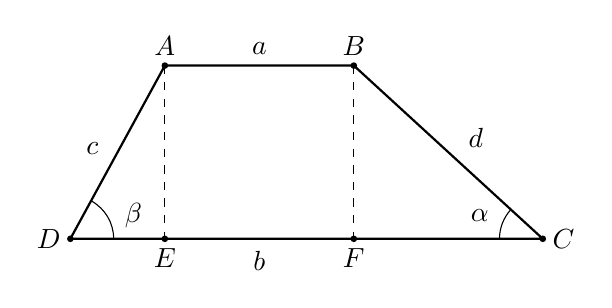
\begin{tikzpicture}[scale=1.0]
  \coordinate (D) at (0,0);
  \coordinate (C) at (6,0);
  \coordinate (A) at (1.2,2.2);
  \coordinate (B) at (3.6,2.2);
  \coordinate (E) at (1.2,0);
  \coordinate (F) at (3.6,0);
  \draw[thick] (D)--(C)--(B)--(A)--cycle;
  \draw[dashed] (A)--(E);
  \draw[dashed] (B)--(F);
  \fill (A) circle (1.2pt) node[above] {$A$};
  \fill (B) circle (1.2pt) node[above] {$B$};
  \fill (C) circle (1.2pt) node[right] {$C$};
  \fill (D) circle (1.2pt) node[left] {$D$};
  \fill (E) circle (1.2pt) node[below] {$E$};
  \fill (F) circle (1.2pt) node[below] {$F$};
  \node at (2.4,2.42) {$a$};
  \node at (2.4,-0.28) {$b$};
  \node at (0.28,1.15) {$c$};
  \node at (5.15,1.28) {$d$};
  % 角 β（D 处，DC 与 DA 之间）
  \draw (0.55,0) arc[start angle=0, end angle=61, radius=0.55];
  \node at (0.80,0.30) {$\beta$};
  % 角 α（C 处，CD 与 CB 之间）
  \draw ([shift={(6,0)}]137:0.55) arc[start angle=137, end angle=180, radius=0.55];
  \node at (5.20,0.30) {$\alpha$};
\end{tikzpicture}
\end{center}
\nopagebreak[4]
由 $a:b:c:d=1:3:1:2$，可设 $a=t$，则 $b=3t$，$c=t$，$d=2t$；下文直接以 $a$ 为单位写出（即取 $t=a$）。

\Needspace{5\baselineskip}
自 $A$、$B$ 分别向 $DC$ 作垂线 $AE$、$BF$，垂足为 $E$、$F$。设 $DE=x$，则

\nopagebreak[4]
\[
FC=DC-DE-EF=3a-a-x=2a-x.
\]

\Needspace{5\baselineskip}
（$EF=AB=a$，因 $AE$、$BF$ 同垂直于 $DC$，$ABFE$ 为矩形。）由勾股定理，

\nopagebreak[4]
\[
AE^2=AD^2-DE^2=c^2-x^2=a^2-x^2,
\]

\nopagebreak[4]
\[
BF^2=BC^2-FC^2=d^2-(2a-x)^2=(2a)^2-(2a-x)^2.
\]

\Needspace{5\baselineskip}
高 $AE=BF$，所以

\nopagebreak[4]
\[
a^2-x^2=(2a)^2-(2a-x)^2
\quad\Longrightarrow\quad
4ax=a^2
\quad\Longrightarrow\quad
x=\frac14a.
\]

\Needspace{5\baselineskip}
于是 $FC=2a-\dfrac14a=\dfrac74a$。在直角三角形中读出各三角函数值：

\nopagebreak[4]
\[
\cos\alpha=\frac{FC}{BC}=\frac{7a/4}{2a}=\frac78,
\]

\nopagebreak[4]
\[
\sin\alpha=\frac{BF}{BC}
=\frac{\sqrt{(2a)^2-(7a/4)^2}}{2a}
=\frac{\sqrt{15}a/4}{2a}
=\frac{\sqrt{15}}8,
\]

\nopagebreak[4]
\[
\sin\beta=\frac{AE}{AD}
=\frac{\sqrt{15}a/4}{a}
=\frac{\sqrt{15}}4.
\]

\gkanswer{答案：$\cos\alpha=\dfrac78$，$\sin\alpha=\dfrac{\sqrt{15}}8$，$\sin\beta=\dfrac{\sqrt{15}}4$。}

\end{answer}
\begin{answer}
\gksolhead{6}{}

\textbf{题目}：

分别在三个平面直角坐标上作出下列方程的图形。

\begin{gktip}
\textbf{题号说明}：原卷本题三个小题印作“1．”“2．”“3．”，本卷按小问格式重排为（1）（2）（3），未增删题干。
\end{gktip}

（1） $(x+2)(y-1)=0$；

（2） $(x+2)^2+(y-1)^2=0$；

（3） $(x+2)^2-(y-1)^2=0$。

\begin{gktip}
\textbf{参考题}
\textbf{源卷说明}：参考题供超过高中水平的高中生做，考生在答完正题后，若有余力应做此题，在总分之外加分，如作正确解答，正题和参考题总分为 120 分。
\textbf{题号说明}：参考题两题的小题原卷印作“1．”“2．”“3．”，本卷按小问格式重排为（1）（2）（3），未增删题干。
\end{gktip}

\textbf{参考题 1．}

（1） 求函数 $f(x)=\frac14x^4-x^3-2x^2+3$ 的极值。（4 分）

\Needspace{5\baselineskip}
（2） 计算

\nopagebreak[4]
\[
\int\left(\frac{1}{\sqrt{1-x^2}}-\frac{x^2}{\sqrt{4-x^2}}\right)dx.
\]

（4 分）

\Needspace{5\baselineskip}
（3） 计算

\nopagebreak[4]
\[
\iint\limits_{(D)}(1+y^2)\,dx\,dy,
\]

其中 $(D)$ 是 $y=x^2$，$x=y^2$ 所围成的区域。（4 分）

\textbf{参考题 2．} 求下列方程的通解：

（1） $x\,dy-2y\,dx=3x^2\,dx$；

（2） $y''-2y'+y=\cos x$。

\Needspace{4\baselineskip}
\textbf{解析}

\gksubpart{（1）}

$(x+2)(y-1)=0$ 要求两因式至少一个为零：$x+2=0$ 或 $y-1=0$，图象为两条直线 $x=-2$ 与 $y=1$：
\nopagebreak[4]
\begin{center}% 1977 年四川卷第六题(1)：(x+2)(y-1)=0 的图象——直线 x=-2 与 y=1（按源卷第 5 页图一布局）
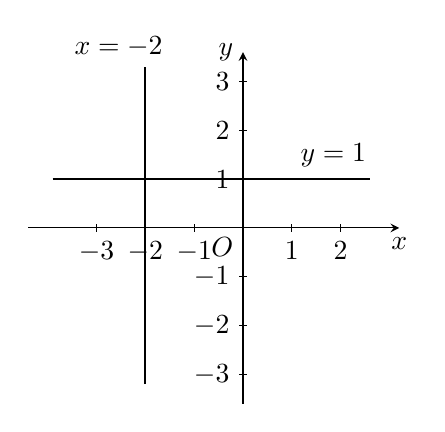
\begin{tikzpicture}[scale=0.62,>=stealth]
  \draw[->] (-4.4,0)--(3.2,0) node[below] {$x$};
  \draw[->] (0,-3.6)--(0,3.6) node[left] {$y$};
  \node[below left] at (0,0) {$O$};
  \foreach \x in {-3,-2,-1,1,2}{
    \draw[thin] (\x,0.08)--(\x,-0.08) node[below] {$\x$};
  }
  \foreach \y in {-3,-2,-1,1,2,3}{
    \draw[thin] (0.08,\y)--(-0.08,\y) node[left] {$\y$};
  }
  \draw[thick] (-2,-3.2)--(-2,3.3);
  \draw[thick] (-3.9,1)--(2.6,1);
  \node[above] at (-2.55,3.30) {$x=-2$};
  \node[above] at (1.85,1.04) {$y=1$};
\end{tikzpicture}
\end{center}
\nopagebreak[4]
\gksubpart{（2）}

$(x+2)^2$ 与 $(y-1)^2$ 均非负，其和为零必须同时为零，故图象为孤立点 $(-2,1)$：
\nopagebreak[4]
\begin{center}% 1977 年四川卷第六题(2)：(x+2)^2+(y-1)^2=0 的图象——孤立点 (-2,1)（按源卷第 5 页图二布局）
\begin{tikzpicture}[scale=0.62,>=stealth]
  \draw[->] (-4.4,0)--(3.9,0) node[below] {$x$};
  \draw[->] (0,-3.6)--(0,3.6) node[left] {$y$};
  \node[below left] at (0,0) {$O$};
  \foreach \x in {-3,-2,-1,1,2,3}{
    \draw[thin] (\x,0.08)--(\x,-0.08) node[below] {$\x$};
  }
  \foreach \y in {-3,-2,-1,1,2,3}{
    \draw[thin] (0.08,\y)--(-0.08,\y) node[left] {$\y$};
  }
  \fill (-2,1) circle (2.2pt);
  \node[above] at (-2,1.15) {$(-2,1)$};
\end{tikzpicture}
\end{center}
\nopagebreak[4]
\gksubpart{（3）}

\Needspace{5\baselineskip}
分解因式：

\nopagebreak[4]
\[
(x+2)^2-(y-1)^2=\bigl[(x+2)+(y-1)\bigr]\bigl[(x+2)-(y-1)\bigr]=(x+y+1)(x-y+3)=0,
\]

图象为两条直线 $x-y+3=0$ 与 $x+y+1=0$（交点恰为 $(-2,1)$）：
\nopagebreak[4]
\begin{center}% 1977 年四川卷第六题(3)：(x+2)^2-(y-1)^2=0 的图象——直线 x-y+3=0 与 x+y+1=0（按源卷第 5 页图三布局）
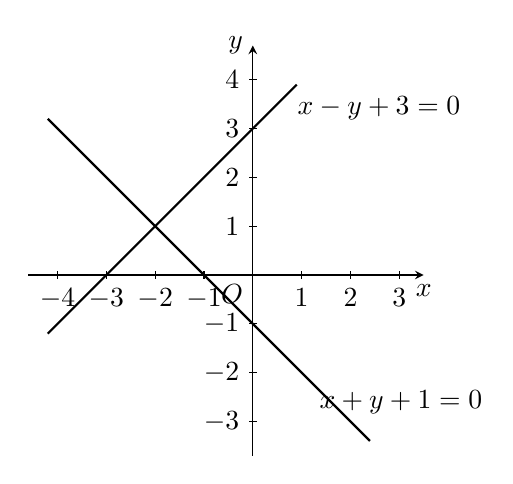
\begin{tikzpicture}[scale=0.62,>=stealth]
  \draw[->] (-4.6,0)--(3.5,0) node[below] {$x$};
  \draw[->] (0,-3.7)--(0,4.7) node[left] {$y$};
  \node[below left] at (0,0) {$O$};
  \foreach \x in {-4,-3,-2,-1,1,2,3}{
    \draw[thin] (\x,0.08)--(\x,-0.08) node[below] {$\x$};
  }
  \foreach \y in {-3,-2,-1,1,2,3,4}{
    \draw[thin] (0.08,\y)--(-0.08,\y) node[left] {$\y$};
  }
  \draw[thick] (-4.2,-1.2)--(0.9,3.9);
  \draw[thick] (-4.2,3.2)--(2.4,-3.4);
  \node[right] at (0.72,3.42) {$x-y+3=0$};
  \node[below right,inner sep=1pt] at (1.30,-2.30) {$x+y+1=0$};
\end{tikzpicture}
\end{center}
\nopagebreak[4]
\textbf{参考题 1}

\gksubpart{（1）}

\nopagebreak[4]
\[
f'(x)=x^3-3x^2-4x=x(x-4)(x+1),
\]

\Needspace{5\baselineskip}
驻点为 $x=0$，$4$，$-1$。二阶导数 $f''(x)=3x^2-6x-4$：

\nopagebreak[4]
\[
f''(0)=-4<0,
\qquad
f''(4)=20>0,
\qquad
f''(-1)=5>0.
\]

所以 $f(x)$ 在 $x=0$ 取极大值 $f(0)=3$；在 $x=4$ 取极小值 $f(4)=-29$；在 $x=-1$ 取极小值 $f(-1)=2\dfrac14$。

\gksubpart{（2）}

\Needspace{5\baselineskip}
第一项是标准积分 $\displaystyle\int\frac{dx}{\sqrt{1-x^2}}=\arcsin x+C_1$。第二项令 $x=2\sin t$，则 $dx=2\cos t\,dt$，$\sqrt{4-x^2}=2\cos t$：

\nopagebreak[4]
\[
\int\frac{x^2}{\sqrt{4-x^2}}\,dx
=\int\frac{4\sin^2t}{2\cos t}\cdot2\cos t\,dt
=\int4\sin^2t\,dt
=\int2(1-\cos2t)\,dt
=2t-\sin2t+C_2.
\]

\begin{gktip}
\textbf{源注}：源解答此处中间步印作 $\int2(1+\cos2t)\,dt$，但其结果 $2t-\sin2t$ 只对应 $1-\cos2t$，系排印失误；本库按 $1-\cos2t$ 计算。
\end{gktip}

\Needspace{5\baselineskip}
代回 $t=\arcsin\dfrac x2$，并用 $\sin2t=2\sin t\cos t=\dfrac x2\sqrt{4-x^2}$：

\nopagebreak[4]
\[
\int\frac{x^2}{\sqrt{4-x^2}}\,dx
=2\arcsin\frac x2-\frac x2\sqrt{4-x^2}+C_2.
\]

\Needspace{5\baselineskip}
所以

\nopagebreak[4]
\[
\int\left(\frac{1}{\sqrt{1-x^2}}-\frac{x^2}{\sqrt{4-x^2}}\right)dx
=\arcsin x-2\arcsin\frac x2+\frac x2\sqrt{4-x^2}+C.
\]

\gksubpart{（3）}
\nopagebreak[4]
\begin{center}% 1977 年四川卷参考题一(3)：抛物线 y=x^2 与 x=y^2 所围区域 (D)（浅灰填充）
% 交点 (0,0) 与 (1,1)，右侧标注 y=x^2、x=y^2、(1,1)，区域内标 D（按源卷第 7 页布局）
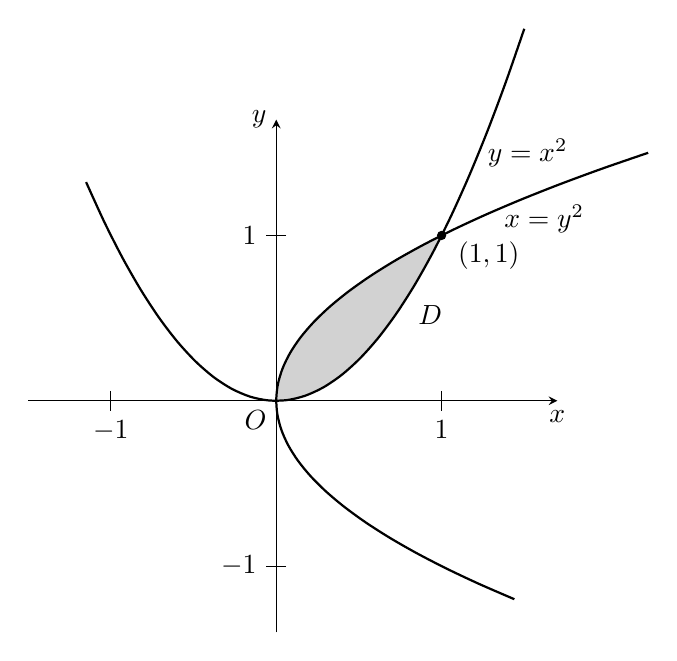
\begin{tikzpicture}[scale=2.1,>=stealth]
  \draw[->] (-1.5,0)--(1.7,0) node[below] {$x$};
  \draw[->] (0,-1.4)--(0,1.7) node[left] {$y$};
  \node[below left] at (0,0) {$O$};
  % 区域 (D)：0≤x≤1 上 y=x²（下）与 y=√x（上）之间
  \fill[gray!35]
    (0,0) plot[domain=0:1,smooth] (\x,{\x*\x})
    -- plot[domain=1:0,smooth] (\x,{sqrt(\x)}) -- cycle;
  \draw[thick,domain=-1.15:1.5,smooth] plot (\x,{\x*\x});
  \draw[thick,domain=-1.2:1.5,smooth,samples=30] plot ({\x*\x},{\x});
  \fill (1,1) circle (0.8pt);
  \node[right] at (1.04,0.88) {$(1,1)$};
  \node[right] at (0.80,0.52) {$D$};
  \node[right] at (1.22,1.50) {$y=x^2$};
  \node[right] at (1.32,1.10) {$x=y^2$};
  \foreach \x in {-1,1}{
    \draw[thin] (\x,0.06)--(\x,-0.06) node[below] {$\x$};
  }
  \foreach \y in {-1,1}{
    \draw[thin] (0.06,\y)--(-0.06,\y) node[left] {$\y$};
  }
\end{tikzpicture}
\end{center}
\nopagebreak[4]
\Needspace{5\baselineskip}
区域 $(D)$ 上 $0\le x\le1$，$x^2\le y\le\sqrt x$。化成先 $y$ 后 $x$ 的累次积分：

\nopagebreak[4]
\[
\iint\limits_{(D)}(1+y^2)\,dx\,dy
=\int_0^1\Bigl(\int_{x^2}^{\sqrt x}(1+y^2)\,dy\Bigr)dx.
\]

\Needspace{5\baselineskip}
内层积分：

\nopagebreak[4]
\[
\int_{x^2}^{\sqrt x}(1+y^2)\,dy
=\Bigl[y+\frac{y^3}3\Bigr]_{x^2}^{\sqrt x}
=\sqrt x+\frac{x^{3/2}}3-x^2-\frac{x^6}3.
\]

\Needspace{5\baselineskip}
外层逐项积分：

\nopagebreak[4]
\[
\int_0^1\Bigl(\sqrt x+\frac{x^{3/2}}3-x^2-\frac{x^6}3\Bigr)dx
=\frac23+\frac2{15}-\frac13-\frac1{21}
=\frac{44}{105}.
\]

\textbf{参考题 2}

\gksubpart{（1）}

\Needspace{5\baselineskip}
当 $x\ne0$ 时，方程可写成

\nopagebreak[4]
\[
\frac{dy}{dx}-\frac2x y=3x.
\]

\Needspace{5\baselineskip}
两边乘以 $x^{-2}$，左端凑成商的导数：

\nopagebreak[4]
\[
x^{-2}\frac{dy}{dx}-2x^{-3}y=\frac{d}{dx}\Bigl(\frac y{x^2}\Bigr)=\frac3x,
\]

\Needspace{5\baselineskip}
积分得

\nopagebreak[4]
\[
\frac y{x^2}=3\operatorname{Ln}|x|+C,
\]

\Needspace{5\baselineskip}
即通解

\nopagebreak[4]
\[
y=3x^2\operatorname{Ln}|x|+Cx^2
\qquad(C\ \text{\text{为任意常数}}).
\]

\gksubpart{（2）}

\Needspace{5\baselineskip}
相应的齐次方程 $y''-2y'+y=0$ 的特征方程为

\nopagebreak[4]
\[
\lambda^2-2\lambda+1=0,
\qquad
\lambda_1=\lambda_2=1,
\]

\Needspace{5\baselineskip}
故齐次通解为 $y=C_1\mathrm e^{x}+C_2x\mathrm e^{x}$。设特解 $y^*=A\cos x+B\sin x$，代入原方程：

\nopagebreak[4]
\[
y^{*\prime\prime}-2y^{*\prime}+y^*
=2A\sin x-2B\cos x=\cos x,
\]

\Needspace{5\baselineskip}
比较系数得 $A=0$，$B=-\dfrac12$，即 $y^*=-\dfrac12\sin x$。所以通解为

\nopagebreak[4]
\[
y=C_1\mathrm e^{x}+C_2x\mathrm e^{x}-\frac12\sin x.
\]

\gkanswer{答案（1）：图象为两条直线 $x=-2$ 与 $y=1$。}

\gkanswer{答案（2）：图象为一个点 $(-2,1)$。}

\gkanswer{答案（3）：图象为两条直线 $x-y+3=0$ 与 $x+y+1=0$。}

\end{answer}